\subsection{UC4 - Gestione delle cartelle sincronizzate}
\begin{figure}[H]
    \centering
    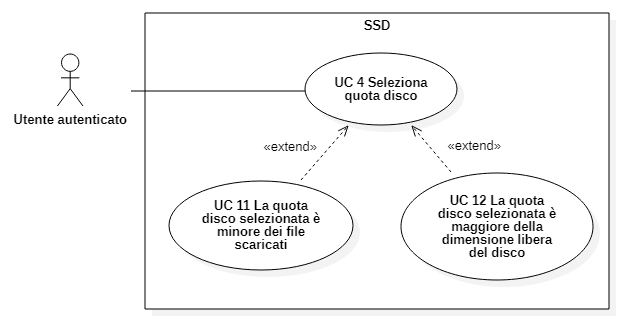
\includegraphics[scale = 0.7]{components/img/UC4.png}
    \caption{UC4 - Gestione delle cartelle sincronizzate}
\end{figure}
\begin{itemize}
\item \textbf{Attore Primario:} Utente autenticato;
\item \textbf{Precondizione:} L'utente ha a disposizione varie funzionalità per la gestione delle cartelle sincronizzate;
\item \textbf{Postcondizione:} Viene eseguita l'operazione richiesta dall'utente;
\item \textbf{Scenario principale:}
    \begin{enumerate}
    \item L'utente può visualizzare l'elenco delle cartelle sincronizzate;
    \item L'utente può aggiungere una cartella da sincronizzare;
    \item L'utente può annullare la sincronizzazione per una cartella;
    \item L'utente può mettere in pausa la sincronizzazione per una cartella;
    \item L'utente può riprendere la sincronizzazione per una cartella.
    \end{enumerate}
\item \textbf{Estensioni:}
\begin{itemize}
\item L'utente cerca di aggiungere una cartella non idonea;
\item L'utente cerca di aggiungere una cartella che ha lo stesso identificativo di una già sincronizzata.
\end{itemize}
\end{itemize}